\documentclass[10pt]{beamer}
\usepackage[utf8]{inputenc}
\usepackage[T1]{fontenc}
\usepackage[spanish]{babel}
\usepackage{amsmath}
\usepackage{amssymb}
\usepackage{graphicx}
\usepackage{algorithm}
\usepackage{algpseudocode}
\usepackage{tikz}
\usepackage{booktabs}
\usepackage{xcolor}

% Configuración del tema
\usetheme{Madrid}
\usecolortheme{default}

% Colores personalizados
\definecolor{azulUni}{RGB}{0,102,204}
\definecolor{grisOscuro}{RGB}{64,64,64}
\definecolor{verdeClaro}{RGB}{46,125,50}

\setbeamercolor{structure}{fg=azulUni}
\setbeamercolor{palette primary}{bg=azulUni,fg=white}
\setbeamercolor{palette secondary}{bg=grisOscuro,fg=white}

% Información del documento
\title[Optimizadores de Gradiente]{Implementación de Técnicas de Descenso de Gradiente Estocástico y Variantes}
\subtitle{Una Comparación Experimental}
\author[Trigueros]{Brandon Trigueros}
\institute[Universidad de Costa Ricas]{Facultad de Ingeniería\\Universidad de Costa Rica}
\date{\today}

% Logo (opcional - descomenta si tienes logo)
%\logo{\includegraphics[height=0.8cm]{logo.png}}

\begin{document}

% Página de título
\begin{frame}
\titlepage
\end{frame}

% Índice
\begin{frame}{Índice}
\tableofcontents
\end{frame}

\section{Introducción}

\begin{frame}{Motivación}
\begin{itemize}
\item El \textbf{descenso de gradiente} es fundamental en optimización y aprendizaje automático
\item Analogía: como una persona caminando por un paisaje de montañas buscando el valle más bajo
\item \textbf{Problema}: El método clásico es muy lento con grandes datasets
\item \textbf{Solución}: Variantes estocásticas más eficientes
\end{itemize}

\begin{center}
\begin{tikzpicture}[scale=0.8]
% Superficie de error simplificada
\draw[thick, blue] plot[smooth, domain=-3:3] (\x, {0.3*\x*\x + 1});
\draw[->] (-3.5,0) -- (3.5,0) node[right] {$\theta$};
\draw[->] (0,0) -- (0,4) node[above] {$J(\theta)$};
% Punto inicial y dirección
\filldraw[red] (2,2.2) circle (2pt) node[above] {inicio};
\draw[->, thick, red] (2,2.2) -- (1.5,1.675) node[midway, above] {$-\nabla J$};
\end{tikzpicture}
\end{center}
\end{frame}

\begin{frame}{Objetivos del Trabajo}
\begin{block}{Objetivo Principal}
Comparar experimentalmente cuatro técnicas de optimización:
\begin{itemize}
\item SGD básico
\item SGD con Momentum  
\item RMSProp
\item Adam
\end{itemize}
\end{block}

\begin{block}{Metodología}
\begin{itemize}
\item Implementación en Python desde cero
\item Experimento con regresión logística
\item Dataset Iris (clasificación binaria)
\item Análisis de curvas de convergencia
\end{itemize}
\end{block}
\end{frame}

\section{Fundamentos Teóricos}

\begin{frame}{Descenso de Gradiente Clásico}
\begin{block}{Fórmula Básica}
$$\boldsymbol{\theta}_{t+1} = \boldsymbol{\theta}_t - \eta \nabla_{\boldsymbol{\theta}} J(\boldsymbol{\theta}_t)$$
\end{block}

\begin{columns}
\begin{column}{0.5\textwidth}
\textbf{Ventajas:}
\begin{itemize}
\item Convergencia estable
\item Garantiza llegar al mínimo (funciones convexas)
\end{itemize}
\end{column}
\begin{column}{0.5\textwidth}
\textbf{Desventajas:}
\begin{itemize}
\item Muy lento con datasets grandes
\item Calcula gradiente completo en cada paso
\end{itemize}
\end{column}
\end{columns}

\vspace{0.5cm}
Donde: $\eta$ = tasa de aprendizaje, $J(\boldsymbol{\theta})$ = función de costo
\end{frame}

\begin{frame}{SGD: Descenso de Gradiente Estocástico}
\begin{block}{Idea Principal}
Usar solo \textbf{una muestra} (o pequeño mini-lote) por iteración:
$$\boldsymbol{\theta}_{t+1} = \boldsymbol{\theta}_t - \eta \nabla_{\boldsymbol{\theta}} \ell(\boldsymbol{\theta}_t; \mathbf{x}_{i(t)}, y_{i(t)})$$
\end{block}

\begin{alertblock}{Trade-off Fundamental}
\begin{itemize}
\item \textcolor{verdeClaro}{\textbf{+}} Mucho más rápido computacionalmente
\item \textcolor{verdeClaro}{\textbf{+}} Permite manejar datasets enormes
\item \textcolor{red}{\textbf{-}} Introduce ruido en las actualizaciones
\item \textcolor{red}{\textbf{-}} Trayectoria más errática
\end{itemize}
\end{alertblock}
\end{frame}

\begin{frame}{SGD con Momentum}
\begin{block}{Analogía Física}
Como una bola rodando que \textbf{acumula velocidad} y mantiene inercia
\end{block}

\begin{block}{Fórmulas}
\begin{align}
\mathbf{v}_t &= \gamma \mathbf{v}_{t-1} + \eta \nabla J(\boldsymbol{\theta}_t) \\
\boldsymbol{\theta}_{t+1} &= \boldsymbol{\theta}_t - \mathbf{v}_t
\end{align}
\end{block}

\begin{columns}
\begin{column}{0.5\textwidth}
\textbf{Beneficios:}
\begin{itemize}
\item Acelera en direcciones consistentes
\item Amortigua oscilaciones
\end{itemize}
\end{column}
\begin{column}{0.5\textwidth}
\textbf{Riesgo:}
\begin{itemize}
\item Puede "pasar de largo" el mínimo
\item Requiere ajuste cuidadoso de $\eta$
\end{itemize}
\end{column}
\end{columns}

\vspace{0.3cm}
Típicamente: $\gamma = 0.9$ (retiene 90\% de la velocidad previa)
\end{frame}

\begin{frame}{RMSProp}
\begin{block}{Problema que Resuelve}
Diferentes parámetros pueden necesitar diferentes tasas de aprendizaje
\end{block}

\begin{block}{Fórmulas}
\begin{align}
E[g_j^2]_t &= \rho E[g_j^2]_{t-1} + (1-\rho) g_{j,t}^2 \\
\theta_{j,t+1} &= \theta_{j,t} - \frac{\eta}{\sqrt{E[g_j^2]_t + \varepsilon}} g_{j,t}
\end{align}
\end{block}

\begin{exampleblock}{Intuición}
\begin{itemize}
\item Si un parámetro tiene gradientes grandes $\Rightarrow$ paso más pequeño
\item Si un parámetro tiene gradientes pequeños $\Rightarrow$ paso más grande
\item \textbf{Adaptación automática} por coordenada
\end{itemize}
\end{exampleblock}

Típicamente: $\rho = 0.9$, $\varepsilon = 10^{-8}$
\end{frame}

\begin{frame}{Adam: Lo Mejor de Dos Mundos}
\begin{block}{Combinación Inteligente}
Adam = Momentum + RMSProp
\end{block}

\begin{block}{Fórmulas (simplificadas)}
\begin{align}
m_{j,t} &= \beta_1 m_{j,t-1} + (1-\beta_1) g_{j,t} \quad \text{(momentum)} \\
v_{j,t} &= \beta_2 v_{j,t-1} + (1-\beta_2) g_{j,t}^2 \quad \text{(normalización)} \\
\theta_{j,t+1} &= \theta_{j,t} - \frac{\eta}{\sqrt{\hat{v}_{j,t}} + \varepsilon} \hat{m}_{j,t}
\end{align}
\end{block}

\begin{block}{¿Por qué es Popular?}
\begin{itemize}
\item Funciona bien "out-of-the-box"
\item Pocos hiperparámetros que ajustar
\item Robusto en muchos problemas
\end{itemize}
\end{block}

Valores por defecto: $\beta_1 = 0.9$, $\beta_2 = 0.999$, $\eta = 0.001$
\end{frame}

\section{Implementación del Experimento}

\begin{frame}{Diseño Experimental}
\begin{block}{Dataset Iris}
\begin{itemize}
\item 150 muestras de flores Iris
\item 4 características: longitud/ancho sépalos y pétalos
\item \textbf{Clasificación binaria}: Versicolor vs. Virginia
\item División: 80\% entrenamiento, 20\% prueba
\end{itemize}
\end{block}

\begin{block}{Modelo: Regresión Logística}
\begin{itemize}
\item Función sigmoide: $h_{\mathbf{w}}(\mathbf{x}) = \frac{1}{1 + e^{-\mathbf{w}^T\mathbf{x}}}$
\item Función de costo: Entropía cruzada binaria
\item Gradiente analítico: $\nabla J = \frac{1}{N}\sum_i (h(\mathbf{x}_i) - y_i)\mathbf{x}_i$
\end{itemize}
\end{block}
\end{frame}

\begin{frame}[fragile]{Implementación en Python}
\begin{block}{SGD Básico}
\begin{verbatim}
for epoch in range(epochs):
    for i in range(N):
        y_pred = sigmoid(np.dot(w, X[i]))
        grad = (y_pred - y[i]) * X[i]
        w = w - lr * grad
\end{verbatim}
\end{block}

\begin{block}{SGD con Momentum}
\begin{verbatim}
v = np.zeros(d)  # velocidad inicial
for epoch in range(epochs):
    for i in range(N):
        grad = compute_gradient(w, X[i], y[i])
        v = gamma * v + lr * grad
        w = w - v
\end{verbatim}
\end{block}
\end{frame}

\begin{frame}{Configuración de Hiperparámetros}
Después de experimentación, se eligieron:

\begin{table}[ht]
\centering
\begin{tabular}{lcc}
\toprule
\textbf{Algoritmo} & \textbf{Tasa de Aprendizaje} & \textbf{Parámetros Adicionales} \\
\midrule
SGD & 0.05 & - \\
SGD + Momentum & 0.03 & $\gamma = 0.9$ \\
RMSProp & 0.05 & $\rho = 0.9$, $\varepsilon = 10^{-8}$ \\
Adam & 0.05 & $\beta_1 = 0.9$, $\beta_2 = 0.999$ \\
\bottomrule
\end{tabular}
\end{table}

\begin{alertblock}{Nota Importante}
Momentum requirió menor tasa de aprendizaje para evitar inestabilidad
\end{alertblock}
\end{frame}

\section{Resultados y Análisis}

\begin{frame}{Curvas de Convergencia}
\begin{center}
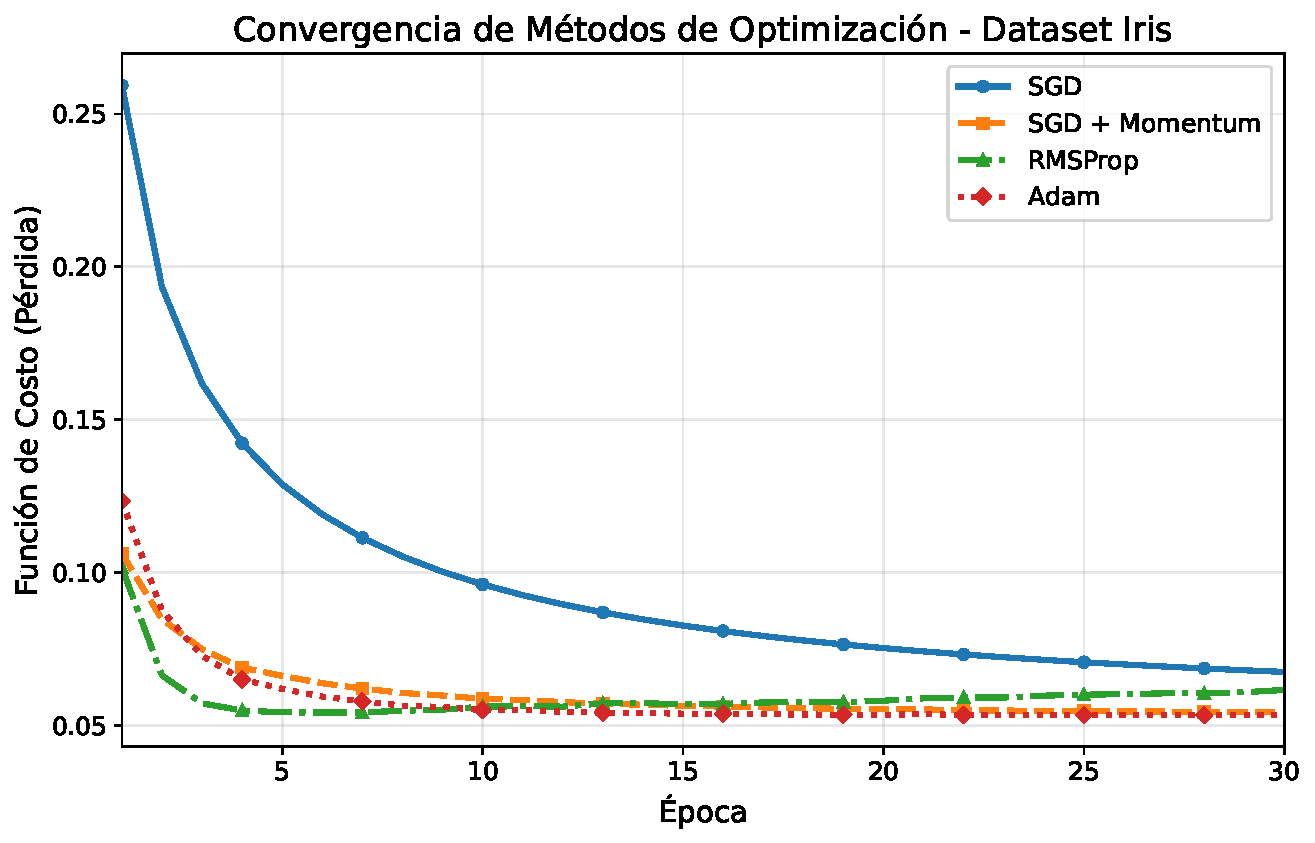
\includegraphics[width=0.85\textwidth]{curvas_convergencia.pdf}
\end{center}

\begin{itemize}
\item \textbf{Adam}: Convergencia más rápida (~5 épocas)
\item \textbf{RMSProp}: Buena velocidad, algo oscilante
\item \textbf{Momentum}: Descenso inicial rápido pero inestable
\item \textbf{SGD}: Más lento pero eventualmente converge
\end{itemize}
\end{frame}

\begin{frame}{Análisis Detallado de Resultados}
\begin{block}{Adam - El Ganador}
\begin{itemize}
\item Pérdida final: $\sim 0.12$ en solo 10 épocas
\item Curva suave y estable
\item Mínima necesidad de ajuste manual
\end{itemize}
\end{block}

\begin{block}{Momentum - Doble Filo}
\begin{itemize}
\item Descenso inicial más drástico (época 2: pérdida $\sim 0.1$)
\item \textcolor{red}{Pero oscilaciones significativas después}
\item Evidencia del problema de "sobrepaso"
\end{itemize}
\end{block}

\begin{block}{RMSProp vs SGD}
\begin{itemize}
\item RMSProp: Convergencia acelerada ($\sim 0.15$ final)
\item SGD: Lento pero confiable ($\sim 0.30$ a época 30)
\end{itemize}
\end{block}
\end{frame}

\begin{frame}{Métricas de Rendimiento Final}
\begin{table}[ht]
\centering
\small
\begin{tabular}{lccc}
\toprule
\textbf{Algoritmo} & \textbf{Costo Final} & \textbf{Precisión Train} & \textbf{Precisión Test} \\
\midrule
SGD & 0.067 & 96.25\% & 95.00\% \\
SGD + Momentum & 0.054 & 96.25\% & 95.00\% \\
RMSProp & 0.062 & 96.25\% & 90.00\% \\
Adam & 0.053 & 97.50\% & 95.00\% \\
\bottomrule
\end{tabular}
\end{table}

\begin{block}{Observaciones Importantes}
\begin{itemize}
\item Precisión final similar en todos los métodos
\item Diferencias principales en \textbf{velocidad de convergencia}
\item Adam ligeramente superior en precisión de entrenamiento
\end{itemize}
\end{block}
\end{frame}

\begin{frame}{Ventajas y Desventajas por Método}
\begin{columns}
\begin{column}{0.5\textwidth}
\begin{block}{SGD}
\textcolor{verdeClaro}{\textbf{Pros:}}
\begin{itemize}
\item Simple de implementar
\item Estable y confiable
\item Buena generalización
\end{itemize}
\textcolor{red}{\textbf{Cons:}}
\begin{itemize}
\item Convergencia lenta
\item Sensible a tasa de aprendizaje
\end{itemize}
\end{block}

\begin{block}{Momentum}
\textcolor{verdeClaro}{\textbf{Pros:}}
\begin{itemize}
\item Acelera convergencia inicial
\item Supera valles estrechos
\end{itemize}
\textcolor{red}{\textbf{Cons:}}
\begin{itemize}
\item Puede oscilar mucho
\item Difícil de calibrar
\end{itemize}
\end{block}
\end{column}

\begin{column}{0.5\textwidth}
\begin{block}{RMSProp}
\textcolor{verdeClaro}{\textbf{Pros:}}
\begin{itemize}
\item Adaptación automática
\item Maneja bien gradientes dispersos
\end{itemize}
\textcolor{red}{\textbf{Cons:}}
\begin{itemize}
\item Algo más complejo
\item Requiere ajuste de $\rho$
\end{itemize}
\end{block}

\begin{block}{Adam}
\textcolor{verdeClaro}{\textbf{Pros:}}
\begin{itemize}
\item Mejor de ambos mundos
\item Funciona "out-of-the-box"
\item Robusto y rápido
\end{itemize}
\textcolor{red}{\textbf{Cons:}}
\begin{itemize}
\item Posible overfitting
\item Mínimos más "afilados"
\end{itemize}
\end{block}
\end{column}
\end{columns}
\end{frame}

\section{Conclusiones}

\begin{frame}{Conclusiones Principales}
\begin{enumerate}
\item \textbf{Adam es el claro ganador} para convergencia rápida y facilidad de uso
\item \textbf{Momentum acelera} pero requiere cuidado en la calibración
\item \textbf{RMSProp} ofrece buen compromiso entre velocidad y estabilidad
\item \textbf{SGD básico} sigue siendo válido para casos que priorizan generalización
\end{enumerate}

\begin{alertblock}{Recomendación Práctica}
\begin{itemize}
\item \textbf{Para empezar}: Adam con parámetros por defecto
\item \textbf{Para ajuste fino}: Considerar híbrido (Adam inicial + SGD final)
\item \textbf{Para datos grandes}: RMSProp o Adam
\item \textbf{Para interpretabilidad}: SGD con momentum controlado
\end{itemize}
\end{alertblock}
\end{frame}

\begin{frame}{Limitaciones y Trabajo Futuro}
\begin{block}{Limitaciones del Estudio}
\begin{itemize}
\item Experimento en problema relativamente simple (Iris)
\item Solo regresión logística (modelo lineal)
\item Conjunto de datos pequeño
\end{itemize}
\end{block}

\begin{block}{Extensiones Propuestas}
\begin{itemize}
\item Probar en redes neuronales profundas
\item Evaluar generalización en datasets más grandes
\item Implementar variantes adicionales (Nadam, AdamW, AMSGrad)
\item Estudiar estrategias de learning rate scheduling
\item Análisis de mínimos "planos" vs "afilados"
\end{itemize}
\end{block}
\end{frame}

\begin{frame}{Impacto en la Práctica}
\begin{block}{En Aprendizaje Automático Moderno}
\begin{itemize}
\item Adam es estándar en deep learning
\item SGD sigue siendo importante para generalización
\item Momentum útil en problemas mal condicionados
\item RMSProp popular en procesamiento de lenguaje natural
\end{itemize}
\end{block}

\begin{exampleblock}{Aplicaciones Reales}
\begin{itemize}
\item \textbf{Visión por computadora}: Adam para entrenar CNNs
\item \textbf{NLP}: RMSProp/Adam para RNNs y Transformers
\item \textbf{Investigación}: SGD para estudios de generalización
\item \textbf{Producción}: Híbridos para mejor rendimiento
\end{itemize}
\end{exampleblock}
\end{frame}

\begin{frame}{Mensajes Clave}
\begin{center}
\Large
\textbf{No existe un optimizador universal}
\end{center}

\vspace{0.5cm}

\begin{itemize}
\item La elección depende del problema específico
\item Adam es un excelente punto de partida
\item Siempre monitorear tanto entrenamiento como validación
\item La implementación correcta es tan importante como la elección del algoritmo
\end{itemize}

\vspace{0.5cm}

\begin{center}
\textcolor{azulUni}{\textbf{El entendimiento teórico guía las decisiones prácticas}}
\end{center}
\end{frame}

\begin{frame}[plain]
\begin{center}
{\Huge \textbf{¿Preguntas?}}

\vspace{1.5cm}

{\Large Gracias por su atención}

\vspace{1cm}

\begin{columns}
\begin{column}{0.5\textwidth}
\centering
Brandon Trigueros\\
\texttt{brandon.trigueros@ucr.ac.cr}
\end{column}
\end{columns}

\vspace{1cm}

{\small Código disponible en: \texttt{github.com/usuario/gradient-descent-research}}
\end{center}
\end{frame}

% Diapositivas de respaldo (opcional)
\appendix

\begin{frame}{Respaldo: Fórmulas Detalladas de Adam}
\begin{block}{Algoritmo Completo}
\begin{align}
m_t &= \beta_1 m_{t-1} + (1-\beta_1) g_t \\
v_t &= \beta_2 v_{t-1} + (1-\beta_2) g_t^2 \\
\hat{m}_t &= \frac{m_t}{1-\beta_1^t} \quad \text{(corrección de sesgo)} \\
\hat{v}_t &= \frac{v_t}{1-\beta_2^t} \quad \text{(corrección de sesgo)} \\
\theta_{t+1} &= \theta_t - \frac{\eta}{\sqrt{\hat{v}_t} + \varepsilon} \hat{m}_t
\end{align}
\end{block}

\begin{itemize}
\item $m_t$: estimación del primer momento (media)
\item $v_t$: estimación del segundo momento (varianza no centrada)
\item Las correcciones de sesgo son importantes en las primeras iteraciones
\end{itemize}
\end{frame}

\begin{frame}{Respaldo: Datos del Experimento}
\begin{table}[ht]
\centering
\footnotesize
\begin{tabular}{c|cccc}
\toprule
\textbf{Época} & \textbf{SGD} & \textbf{Momentum} & \textbf{RMSProp} & \textbf{Adam} \\
\midrule
1 & 0.259 & 0.106 & 0.102 & 0.124 \\
2 & 0.193 & 0.085 & 0.067 & 0.088 \\
5 & 0.129 & 0.066 & 0.054 & 0.062 \\
10 & 0.099 & 0.058 & 0.055 & 0.054 \\
20 & 0.078 & 0.053 & 0.060 & 0.053 \\
30 & 0.068 & 0.054 & 0.062 & 0.053 \\
\bottomrule
\end{tabular}
\caption{Evolución del costo de entrenamiento}
\end{table}

\begin{itemize}
\item Adam converge más rápido en las primeras épocas
\item Momentum muestra la mayor reducción inicial pero luego oscila
\item SGD mejora de manera más gradual y consistente
\end{itemize}
\end{frame}

\end{document}
